\section{Metody interpolacyjne}
\subsection{Regula falsi}
\begin{frame}{Metody interpolacyjne - Regula falsi}
	\centering   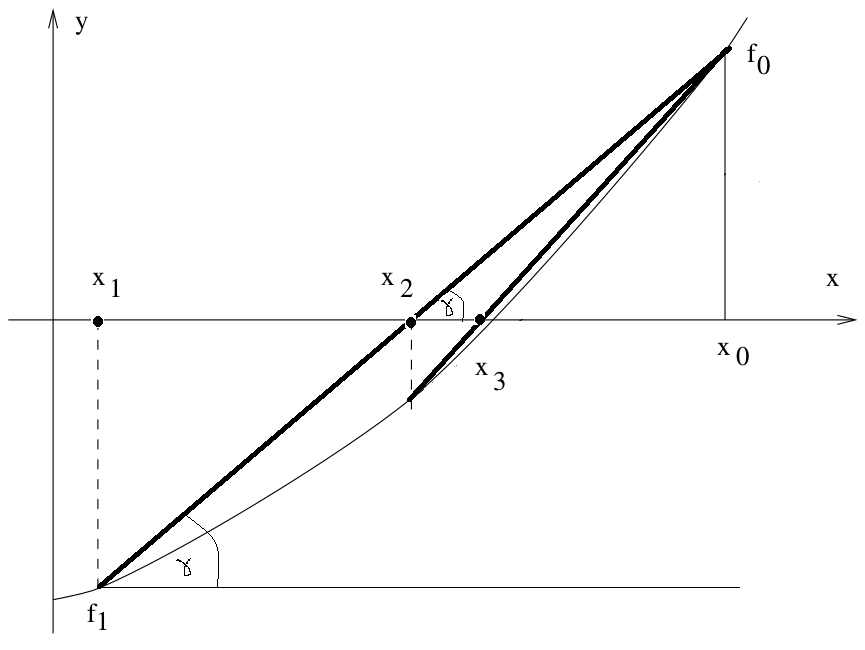
\includegraphics[width=.7\linewidth]{img/7/7_6_3d.png}
\end{frame}
\subsection{Regula falsi}
%%%%%%%%%%%%%%
\begin{frame}{Regula falsi}
	\begin{enumerate}
		\item Startujemy mając punkty $x_{0}$, $x_{1}$ takie, że $f(x_{0}) \cdot f(x_{1}) < 0$
		
		\item przez punkty $x_0$ i $x_1$ prowadzimy prostą i znajdujemy jej punkt przecięcia $x_2$ z osią OX: $\frac{f(x_0) - f(x_1)}{x_{0} - x_{1}} = \frac{f(x_0)}{x_{0} - x_{2}} \Rightarrow x_{2} = \frac{f(x_1)}{f(x_1) - f(x_0)} x_{0} + \frac{f(x_0)}{f(x_0) - f(x_1)}x_{1}$
		
		\item sprawdzamy po której stronie osi OX znajduje się $f(x_2)$ Punkty do kolejnej interacji wybieramy tak, aby leżały po różnych stronach osi OX:
		$ \left
		\begin{array}{ll}
								f(x_1) \cdot f(x_2) < 0\\
								f(x_0) \cdot f(x_2) < 0
							\end{array}\right\} \Rightarrow x_{3} \ldots$\\
	\end{enumerate}
	- wolno zbieżna do poj. pierwiastka (zbieżność liniowa)
\end{frame}
%%%%%%%%%%%%%%
\begin{frame}{Regula falsi}
	Wyjątkowo trudny przypadek:\linebreak
	\begin{center}
		\includegraphics[width=.65\linewidth]{img/7/7_6_2}
	\end{center}
 wszystkie iteracje po tej samej stronie pierwiastka
\end{frame}
%%%%%%%%%%%%%%
\subsection{Metody Illinois i Pegasus - ulepszenie RF}
\begin{frame}{Metody Illinois i Pegasus - ulepszenie RF}
	\begin{enumerate}
	
		\item Jeśli mamy $x_{i}$, $x_{i+1}$, $x_{i+2}$ takie że 
		$\begin{cases}
			f(x_{i}) \cdot f(x_{i+1}) \qquad <0 $ $ \leftarrow $ obejmują pierwiastek\\
			$f(x_{i+1}) \cdot f(x_{i+2}) \quad >0$ 
		$\end{cases}$\\
		Czyli najnowsza wartość $f(x_{i+2})$ jest po tej samej  stronie osi OX co poprzednia 	$f(x_{i+1})$
		\item stosujemy RF korzystając ze starszego punktu $x_{i}$, czyli dla punktów $x_{i}$, $x_{i+2}$  ale ze zmodyfikowaną starszą wartością : $f(x_{i}) = f(x_{i})^{*} = \alpha \cdot f(x_{i})$
		
		\item podobnie gdy\\ $f_{i+2} \cdot f_{i+3}$ $\begin{cases}
			< 0 $ - RF dla $ x_{i+2}$, $ x_{i+3}\\
			> 0 $ - zmodyfikowana RF dla $ x_{i+1}$, $x_{i+3}
		\end{cases}$
	\end{enumerate}
\end{frame}
%%%%%%%%%%%%%%
\begin{frame}{Metody Illinois i Pegasus - ulepszenie RF}
	\centering 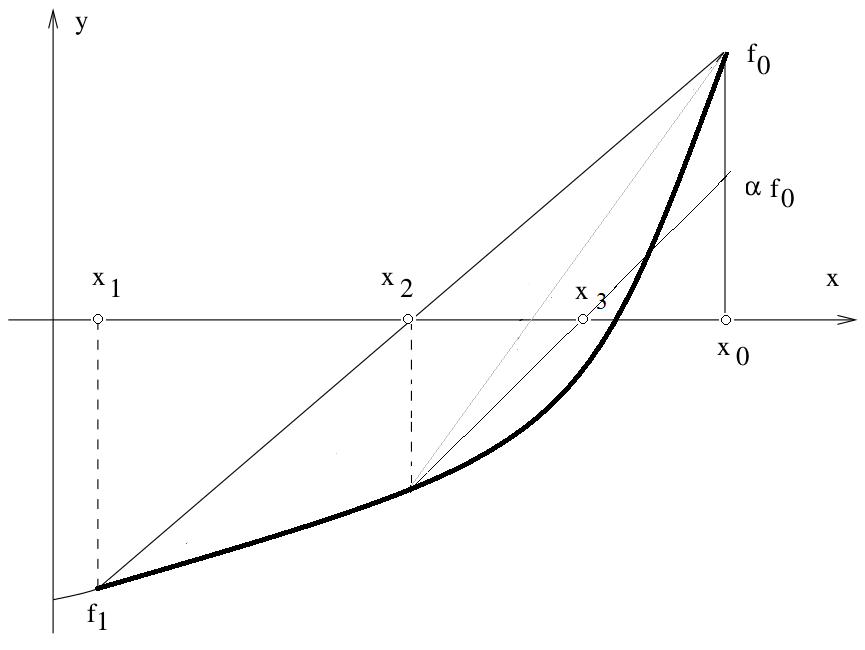
\includegraphics[width=.7\linewidth]{img/7/7_6_3-1} \linebreak
	\textbf{Illinois} $\rightarrow$ $\alpha = \frac{1}{2}$, \quad \textbf{Pegasus} $\rightarrow$ $\alpha = \frac{f_{0}}{f_{1} + f_{0}}$
\end{frame}
%%%%%%%%%%%%%%
\subsection{Metoda siecznych}
\begin{frame}{Metoda siecznych}
	\centering \includegraphics[width=.8\linewidth]{img/7/7_6_4}
\end{frame}
%%%%%%%%%%%%%%
\begin{frame}{Metoda siecznych}
	- startujemy z $(x_{0}, x_{1})$\linebreak
	- $f_{0} \cdot f_{1}$ - nie badamy\linebreak
	linie prosta $(x_{0}, f_{0})$, $(x_{1}, f_{1})$ $\ldots$
	\[
		x_{i+2} = x_{i+1} - \underbrace{\frac{x_{i+1} - x_{i}}{f_{i+1} - f_{i}}}_{(*)} \cdot f_{i+1}
	\]
 Dziala jak N-R, ale z przybliżoną wartością $f'(x_{i})$ za pomocą ilorazu różnicowego 	$(*)$  \linebreak\linebreak
	- rząd zbieżności $\sim$ 1.62 \hspace{5cm} \linebreak
	- lepsza od RF\linebreak
	- gorsza od NR - lecz nie trzeba znać $f'$ !
\end{frame}
\begin{frame}{Metoda Steffensena}
	$$
		 x_{i+1} = x_{i} - \frac{f(x_{i})}{g(x_{i})}
	$$
	gdzie $g(x_i)$ to 
 przybliżenie pochodnej poprzez iloraz różnicowy  $$\frac{f(x_i + f(x_i)) - f(x_i)}{f(x_i)}$$
  
 \begin{itemize}
 \item budujemy sieczną uzywając $x_i$, oraz $x_i+f(x_i)$
 \item $x_{i+1}$ to punkt przecięcia tej siecznej z osią OX
 \item w kolejnym kroku budujemy  sieczną używając $x_{i+1}$ oraz $x_{i+1}+f(x_{i+1})$
     \item  każdy krok wymaga policzenia dwóch nowych wartości funkcji (w metodzie siecznych od drugiego kroku tylko jednej) 
     \item rząd zbieżności =2 (lepszy od metody  siecznych)
 \end{itemize}
\end{frame}
